\begin{frame}{IOTA}
    \begin{columns}
    \column{0.46\linewidth}
        \begin{block}{What Is IOTA?}
            \begin{itemize}
                \item \textbf{Distributed Ledger Technology} for \textbf{Internet-Of-Things} scenarios
                \item Leverages a \textbf{Directed Acyclic Graph} data structure (the \textbf{Tangle})
            \end{itemize}
        \end{block}
        
        \vspace{5pt}
        
        \begin{block}{Main Advantages}
            \begin{itemize}
                \item Cheap \textbf{Proof-Of-Work}, suitable for big data from sensors
                \item \textbf{Scales} well with intense activity
                \item \textbf{Feeless} transactions
                \item \textbf{Public} devnet opened for developers and testing purposes
                \item Well-documented \textbf{APIs} and frameworks
            \end{itemize}
        \end{block}
        
    \column{0pt}
        
    \column{0.46\linewidth}
        \raggedleft
        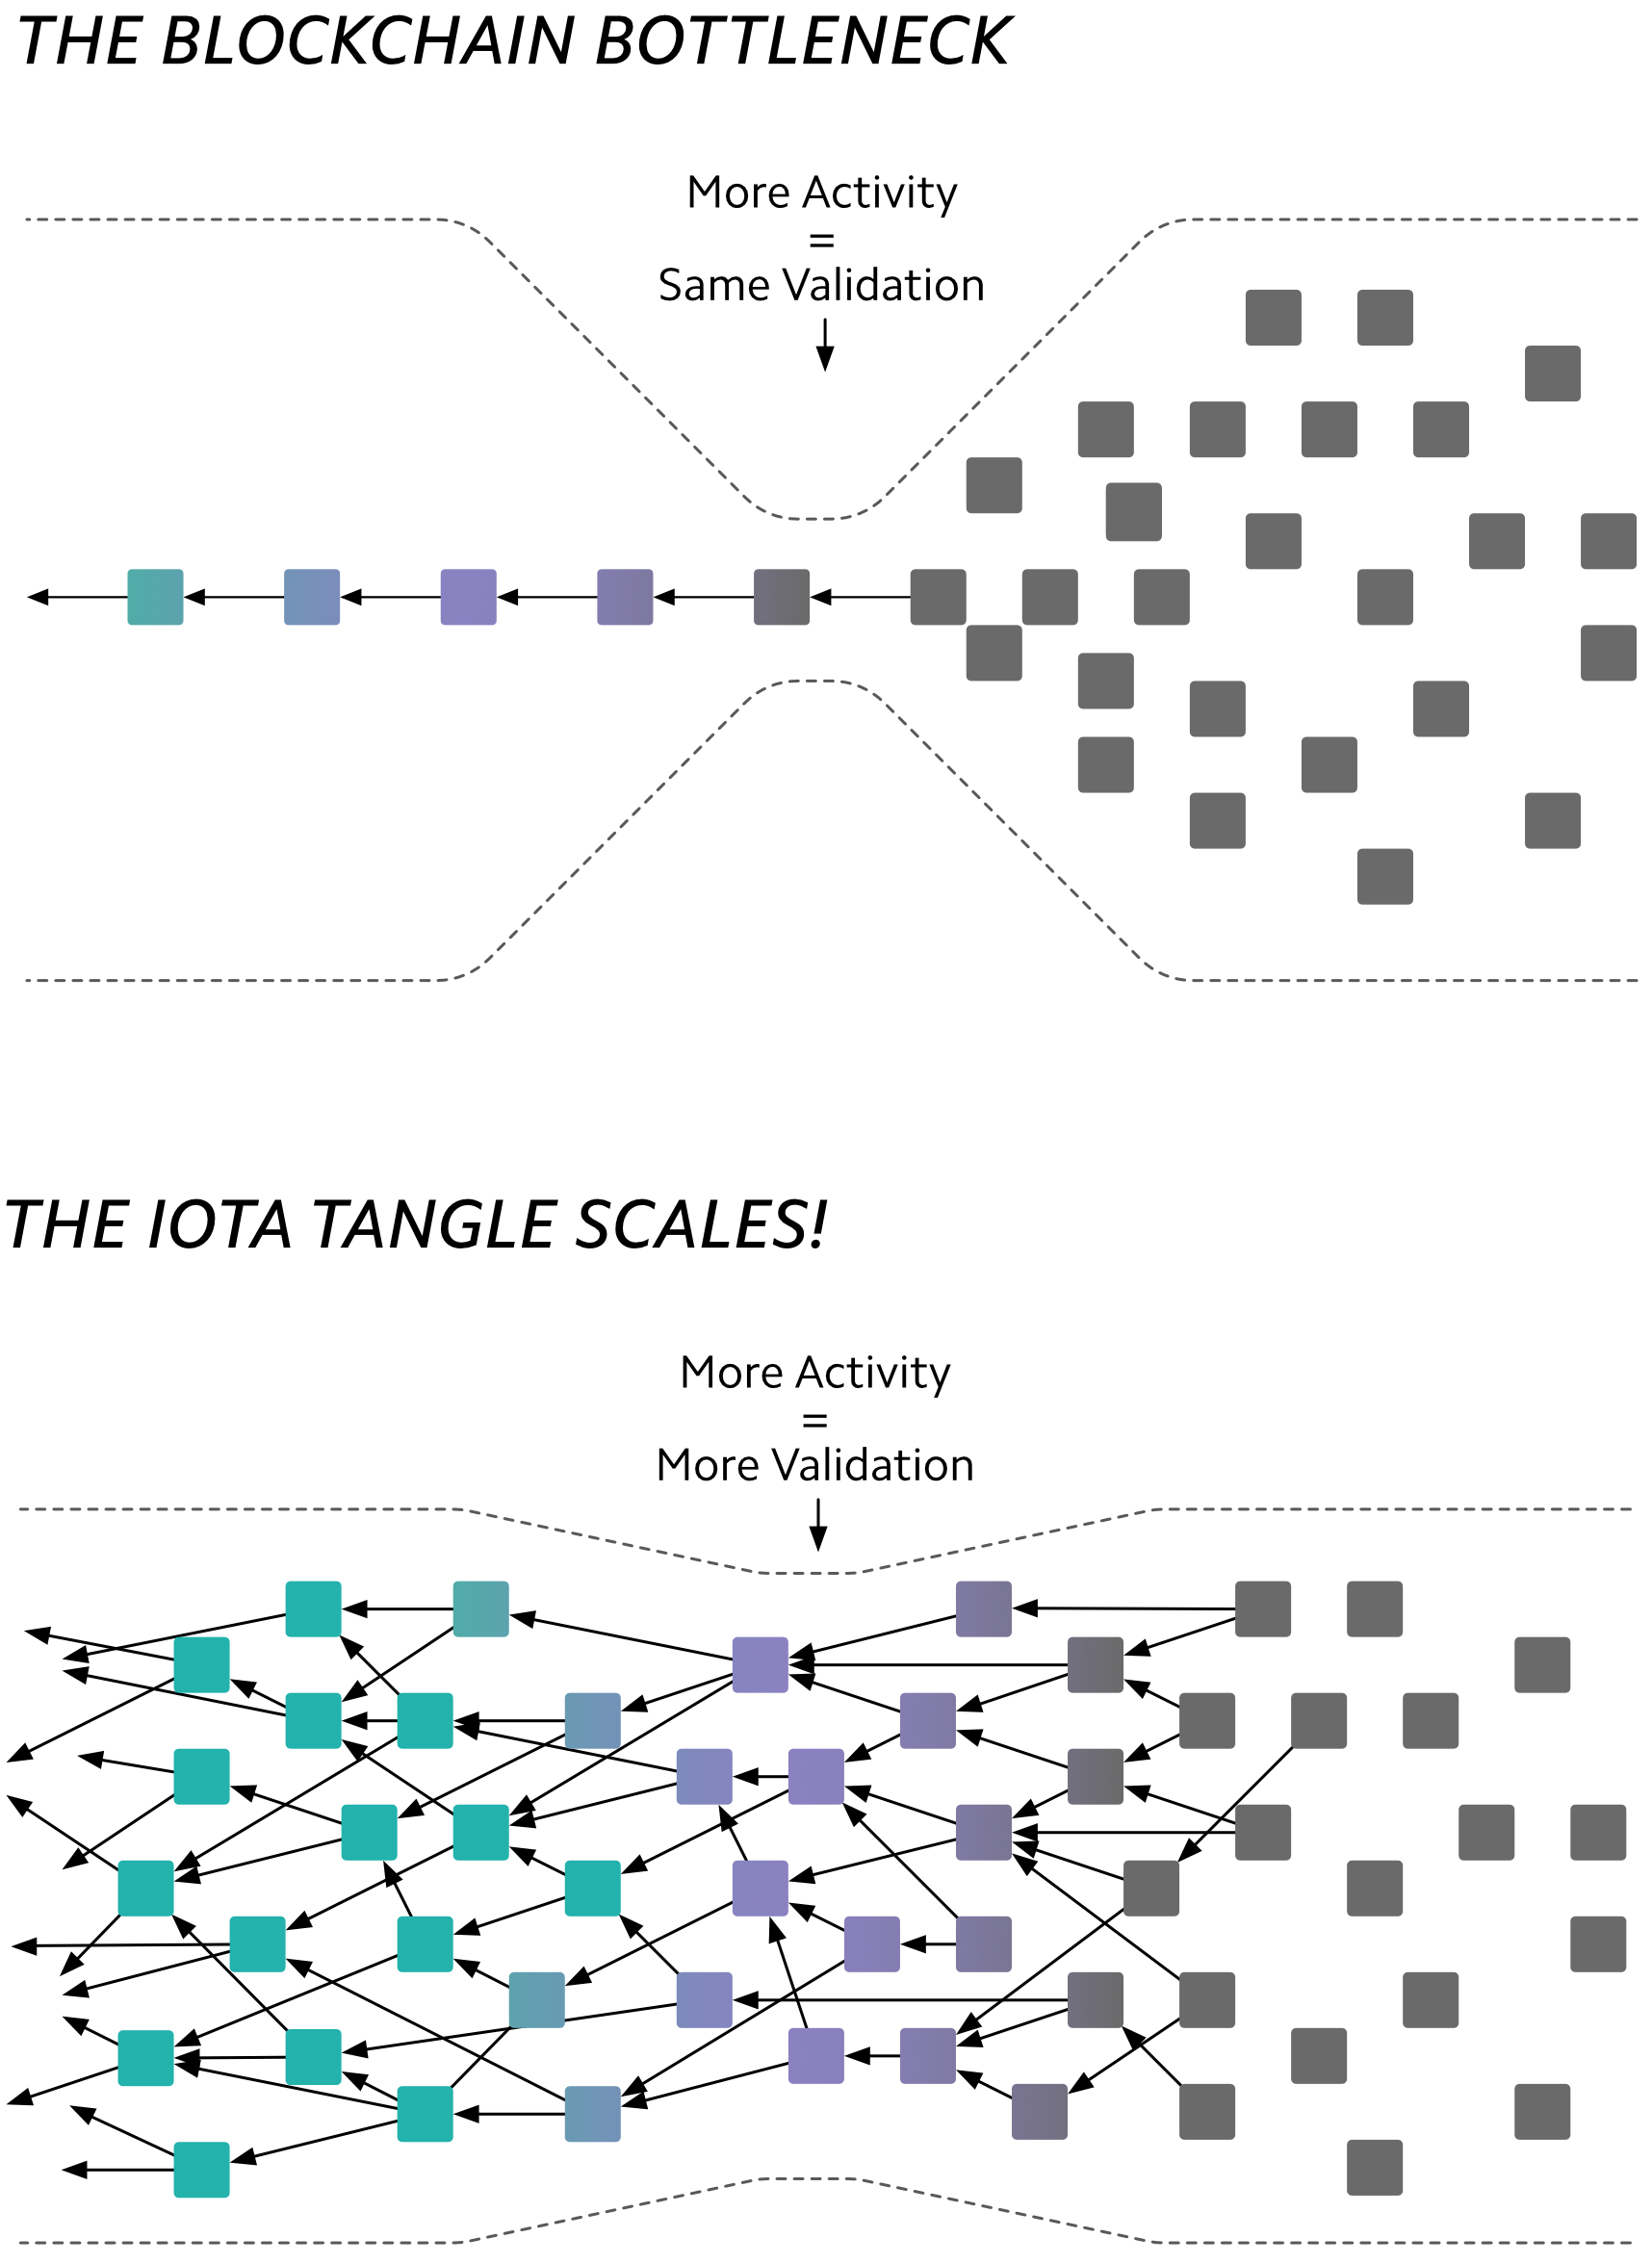
\includegraphics[width = \linewidth]{images/tangle.png}
    \end{columns}
\end{frame}

\begin{frame}{IOTA}
    \begin{columns}[T]
        \column{0.47\linewidth}
        \begin{block}{IOTA Limitations}
            \begin{itemize}
                \item The Tangle provides \textbf{no high-level organisation} for the data
                \item Transaction can be retrieved by tag but not by date of publications
                \begin{itemize}
                    \item [$\Rightarrow$] this can lead to a waste of time
                    \item [$\Rightarrow$] e.g., in our case the geosolver would have to download the same transactions from the tangle every time it is run
                \end{itemize}
            \end{itemize}
        \end{block}
        \centering
        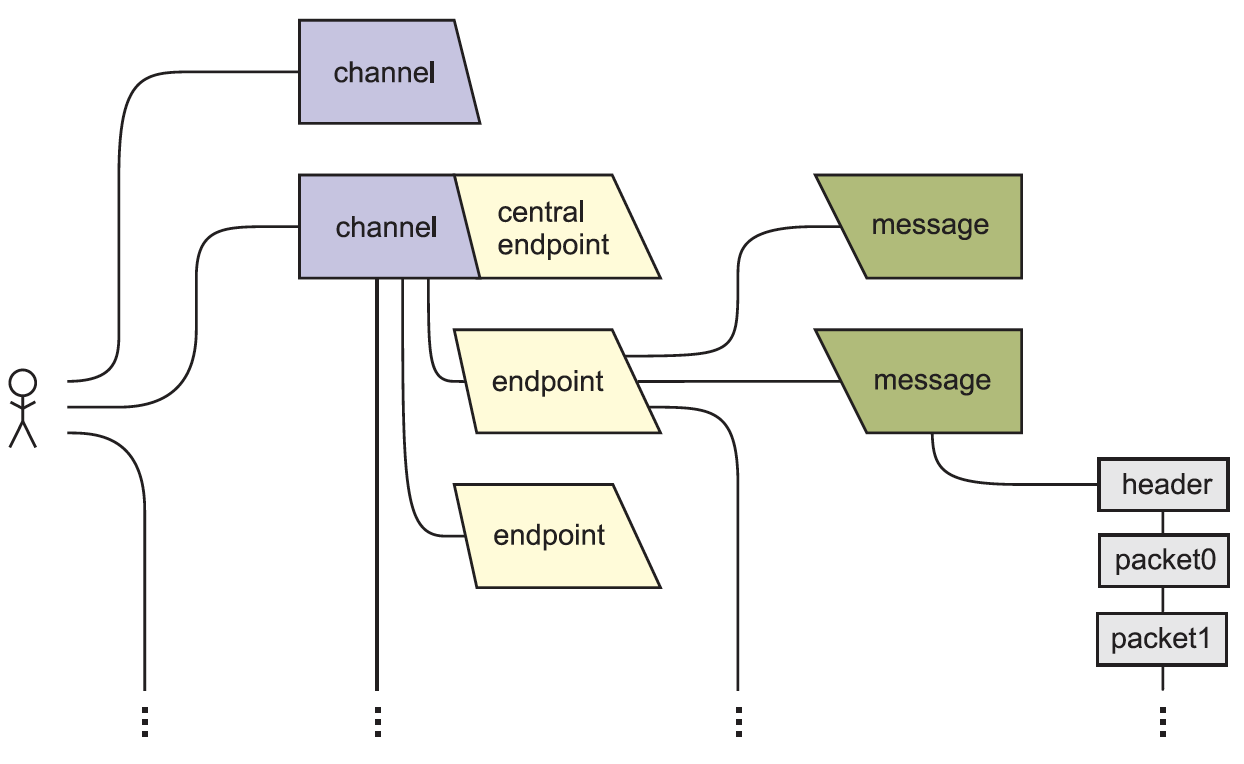
\includegraphics[width=\linewidth]{images/mam.png}
    
        \column{0.47\linewidth}
        \begin{block}{Mam Channels}
            \begin{itemize}
                \item \textbf{Mam Channels} -- or \textit{\textbf{Streams}}, in the new release of IOTA -- represent an "\textbf{abstract layer}" upon the Tangle
                \item Each channel has a root transaction, and each transaction maintains the link to the next root, thus it is possible to append a new message to the channel
                \item Given a root, it is possible to fetch all the subsequent messages as if they were part of a linked list
                \item There is already an API to use Mam Channels in IOTA, as well as an "inspector" at the link: \url{explorer.iota.org/devnet/streams/0/}
            \end{itemize}
        \end{block}
    \end{columns}
\end{frame}

\begin{frame}{IOTA}
    \centering
    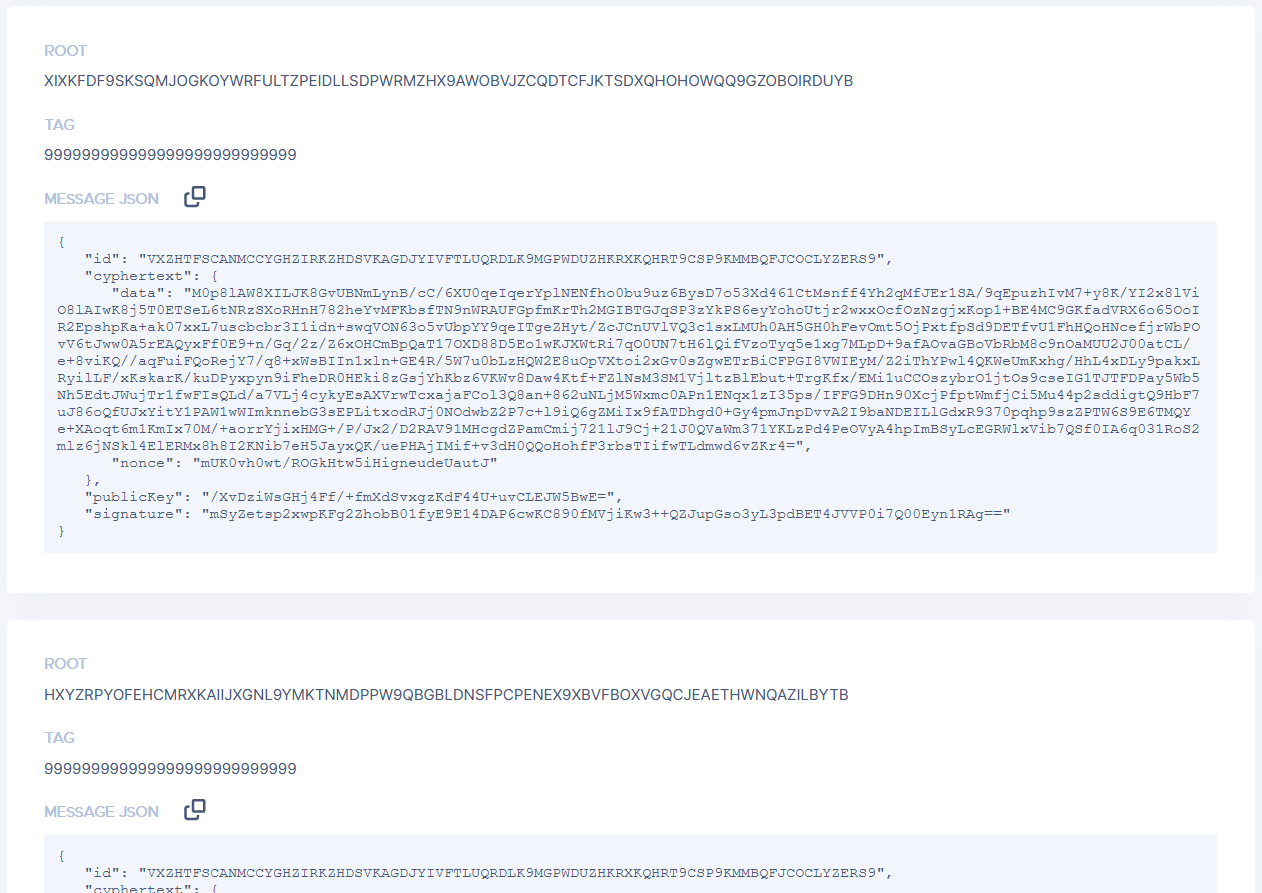
\includegraphics[width=0.85\linewidth]{images/channel.png}\\
    \footnotesize{Example of the Mam Channel of an agent inspected with the IOTA explorer.}
\end{frame}